\section{Theory of 6-poles: classes and transfer relations}\label{sec:theory6}

\paragraph{The 64 classes.} Write $Q = \mathbb{F}_2^{E(\PG)}/\Cut(\PG)$, and call the class in $Q$ of
the sum of the indicator vectors of a multiset of labels the class of that multiset. The cut space
is a binary $[15, 9, 3]$ code (its nonzero words of weight at most 4 are those of
Lemma~\ref{lem:smallcuts}), so $Q$ has 64 elements. A vertex is good exactly when the class of its
three labels is $0$ and they are distinct. The automorphism group of $\PG$ acts on $Q$ with six
orbits (Table~\ref{tab:classes}, Figure~\ref{fig:orbits}); we call them $\Oz$, $\OEc$, $\ODthree$,
$\ODtwo$, $\OTone$, $\OTtwo$. The orbit $\OTone$ is the class of the
all-ones vector: removing from $E(\PG)$ the twelve edges at the four 2-subsets containing a fixed
element of $\{1, \dots, 5\}$ leaves three pairwise antipodal edges (at distance 3 in the line graph),
and these five \emph{antipodal triples} partition $E(\PG)$. The coset-leader weights of the 64 classes are
$0$ (one class), $1$ (fifteen), $2$ (forty-five) and $3$ (three), so the covering radius of the code is 3.

\begin{table}[t]\centering\small
\begin{tabular}{lccl}
\toprule
orbit & classes & least weight & elements of least weight \\
\midrule
$\Oz$ & 1 & 0 & the cut space, containing the ten stars \\
$\OEc$ & 15 & 1 & one edge; also two edges at distance 1 \\
$\ODthree$ & 15 & 2 & two edges at distance 3 \\
$\ODtwo$ & 30 & 2 & two edges at distance 2 (two such pairs per class) \\
$\OTone$ & 1 & 3 & the five antipodal triples \\
$\OTtwo$ & 2 & 3 & triples of pairwise distance-2 edges (ten per class) \\
\bottomrule
\end{tabular}
\caption{The orbits of $\mathrm{Aut}(\PG)$ on the 64 classes modulo the cut space, from the coset table of the cut code
(\texttt{cut\_code\_cosets.json}) and checked against Lemma~\ref{lem:distance}: the number of classes in the orbit, the least
weight of a vector in the class, and the vectors of that weight.}\label{tab:classes}
\end{table}

\begin{figure}[t]\centering
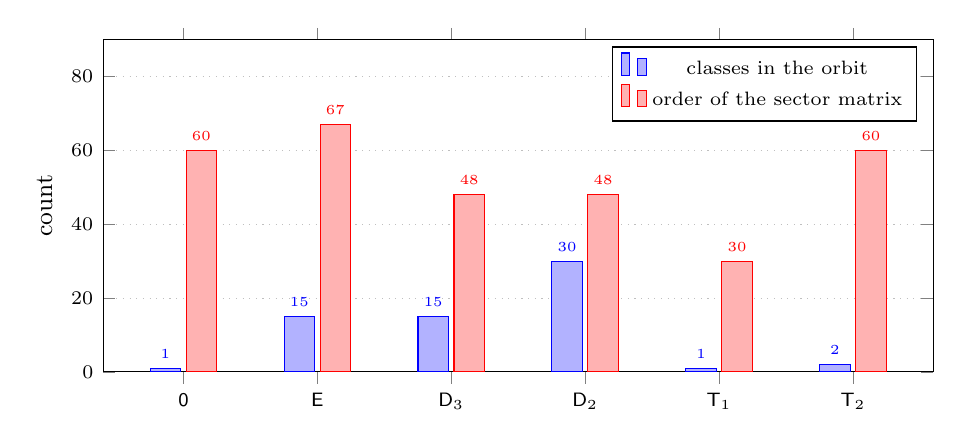
\begin{tikzpicture}
\begin{axis}[ybar,width=\textwidth,height=5.8cm,bar width=11pt,ymin=0,ymax=90,symbolic x coords={0,E,D3,D2,T1,T2},xtick=data,xticklabels={$\mathsf{0}$,$\mathsf{E}$,$\mathsf{D}_3$,$\mathsf{D}_2$,$\mathsf{T}_1$,$\mathsf{T}_2$},ylabel={count},tick label style={font=\scriptsize},label style={font=\small},legend style={font=\scriptsize,at={(0.98,0.98)},anchor=north east},enlarge x limits=0.12,nodes near coords,nodes near coords style={font=\tiny},point meta=y,ymajorgrids=true,grid style={dotted}]
\addplot coordinates {(0,1) (E,15) (D3,15) (D2,30) (T1,1) (T2,2)};
\addplot coordinates {(0,60) (E,67) (D3,48) (D2,48) (T1,30) (T2,60)};
\legend{classes in the orbit,order of the sector matrix}
\end{axis}
\end{tikzpicture}

\caption{The six orbits of the 64 classes modulo the cut space (bars: classes per orbit, from \texttt{cut\_code\_cosets.json}) with the order
of the sector matrix of each orbit (bars: ordered label triples of one representative class, from \texttt{blocks.json}); the orders
satisfy $60 + 15\cdot 67 + 15 \cdot 48 + 30\cdot 48 + 30 + 2\cdot 60 = 15^3$.}\label{fig:orbits}
\end{figure}

\paragraph{6-poles.} A \emph{6-pole} has six dangling ends, split into two connectors of three. The
proof of Lemma~\ref{lem:conduction} shows that a map with every vertex good puts the same class on
both connectors, and the \emph{conducted set} $D(M) \subseteq Q$ is the set of these classes; it
is invariant under $\mathrm{Aut}(\PG)$, hence a union of orbits. Theorem~\ref{thm:ring} holds
verbatim for rings of 6-poles joined along their connectors by three edges, and such rings can be
cyclically 5-edge-connected, since two arcs of a ring are separated by six edges. For a graph $G$
without a Petersen coloring and non-adjacent vertices $u$, $w$, the 6-pole $G - u - w$ with the
ends at $u$ and at $w$ as connectors does not conduct $\Oz$, by the argument of
Lemma~\ref{lem:restore}: class $\Oz$ at the ends of $u$ means three labels forming a star, so restoring $u$
makes it good, and the same class at $w$ makes $w$ good.

\paragraph{Transfer relations.} A \emph{block} is a 6-pole whose connectors $L$ and $R$ are ordered.
Its transfer relation is the set $T_M$ of pairs $(\sigma(L), \sigma(R)) \in E(\PG)^3 \times E(\PG)^3$
over all maps $\sigma$ with every vertex good. In a ring of blocks $M_1, \dots, M_t$, end $j$ of $R_i$
is joined to end $\pi_i(j)$ of $L_{i+1}$ (indices modulo $t$). Every vertex of the ring lies in one
block, so a Petersen coloring of the ring is a labelling of the $3t$ joining edges accepted by
every block: the ring is Petersen colorable if and only if the boolean matrix product
\begin{equation}\label{eq:ringproduct}
T_{M_1} \Pi_1\, T_{M_2} \Pi_2 \cdots T_{M_t} \Pi_t
\end{equation}
has a nonzero diagonal entry, where $\Pi_i$ is the permutation matrix of $\pi_i$.

\begin{proposition}[\claim{D}]\label{prop:sectors}
For $q \in Q$ let $S_q$ be the set of ordered label triples of class $q$.
\begin{enumerate}
\item[\textup{(a)}] $T_M \subseteq \bigcup_{q \in Q} S_q \times S_q$, and every $\Pi_i$ maps each $S_q$
onto itself, so every product of transfer relations and junctions is block diagonal over $Q$.
\item[\textup{(b)}] The diagonal blocks of such a product over two classes of one orbit are conjugate,
so they have the same trace.
\end{enumerate}
Hence a ring is Petersen colorable if and only if, for some orbit, the product of the restrictions
to $S_q \times S_q$, for one fixed class $q$ of that orbit, has a nonzero diagonal. These six
\emph{sector matrices} have orders $60, 67, 48, 48, 30, 60$.
\end{proposition}

\begin{proof}
(a) is the conduction property, and the class of a triple does not depend on the order of its
entries. (b) An automorphism $\alpha$ of $\PG$ maps a map $\sigma$ of $M$ to the map $\alpha \circ
\sigma$, so $(x, y) \in T_M$ if and only if $(\alpha x, \alpha y) \in T_M$; $\alpha$ acts on labels
and $\Pi_i$ on positions, so they commute, and $\alpha$ conjugates the block over $q$ to the block
over $\alpha(q)$. The sector orders add up to $60 + 15 \cdot 67 + 15 \cdot 48 + 30 \cdot 48 + 30 + 2
\cdot 60 = 15^3$, the number of ordered label triples, as they must when the 64 classes partition them:
\begin{equation}\label{eq:sectors}
\sum_{o}\,|o|\cdot n_o \;=\; 60 + 15\cdot 67 + 15\cdot 48 + 30\cdot 48 + 30 + 2\cdot 60 \;=\; 3{,}375 \;=\; 15^3 ,
\end{equation}
with $|o|$ the number of classes in the orbit $o$ and $n_o$ the order of its sector matrix.
\end{proof}

A block is therefore stored as six boolean matrices with $\sum_o n_o^2 = \nBitsPerElement$ entries, and a
product of two blocks costs $\sum_o n_o^3 = \nCubeSum$ multiply-add operations on boolean entries.

\begin{corollary}[\claim{D}]\label{cor:semigroup}
Let $\mathcal{F}$ be a finite set of blocks and $\mathcal{G}$ the set of six-tuples of sector
matrices of $T_M \Pi$, for $M \in \mathcal{F}$ in either orientation and $\pi$ any bijection. Every
ring of at least two blocks of $\mathcal{F}$ is Petersen colorable if and only if every product of at
least two elements of $\mathcal{G}$ has a nonzero diagonal in some sector. This holds if there is a
set $\mathcal{C}$ of six-tuples of boolean matrices such that every product of two elements of
$\mathcal{G}$ contains an element of $\mathcal{C}$ entrywise, every product $cg$ with $c \in
\mathcal{C}$ and $g \in \mathcal{G}$ contains an element of $\mathcal{C}$, and every element of
$\mathcal{C}$ has a nonzero diagonal in some sector; and such a set exists whenever the condition
holds (take all products).
\end{corollary}

\begin{proof}
The first statement is Proposition~\ref{prop:sectors}. For the second, boolean products are
monotone under entrywise containment, so by induction on the length every product of at least two
elements of $\mathcal{G}$ contains an element of $\mathcal{C}$, and its diagonal is nonzero where
that element's is. The set of all products is finite, which gives the converse.
\end{proof}

A set $\mathcal{C}$ as in Corollary~\ref{cor:semigroup} is a \emph{certificate} that can be checked, once regenerated by the commands of Section~\ref{sec:repro}, by
products of boolean matrices of order at most 67 (Algorithm~\ref{alg:check}). The number of generators is
at most $2 \cdot 6 \cdot |\mathcal{F}|$ (two orientations and six junction permutations per block), fewer when
distinct choices give the same matrices.

\begin{lemma}[soundness of computed matrices, \claim{D}]\label{lem:soundness}
Let $\tilde T \subseteq T$ be sector matrices in which every entry is a map accepted by the star-condition
checker. Then every product of the $\tilde T$ and junctions is entrywise contained in the corresponding product
of the exact matrices. A nonzero diagonal entry of a product of computed matrices proves that the ring is
Petersen colorable; a zero diagonal of a product of computed matrices proves nothing unless the computed matrices are
complete.
\end{lemma}

\begin{proof}
Boolean products are monotone under entrywise containment, and a diagonal entry of the contained product is a diagonal
entry of the exact one. The converse fails because a missing entry can turn a nonzero diagonal into a zero one.
\end{proof}

Lemma~\ref{lem:soundness} separates the claims of Section~\ref{sec:results6} into two kinds. The statements
``every ring of these blocks is Petersen colorable'' rest only on soundness. The statements that a sector has a
\emph{zero} diagonal, such as the junction classes of flower snarks (Corollary~\ref{cor:flower}) and the zero diagonals
of the control of Section~\ref{sec:ablation}, rest on the completeness of the computed matrices as well; the completeness
checks of Section~\ref{sec:design} state which matrices have them.

\paragraph{Claws and Petersen superedges.} The \emph{claw} $Y$ is the block with a center joined to
three vertices, each of which carries one dangling end in $L$ and one in $R$. The \emph{Petersen
superedge} $S$ is $\PG - u - w$ with $u$, $w$ at distance 2, $L$ the three ends at $u$ and $R$ the
three ends at $w$; it is the superedge $(P_{10})_{u,v}$ of Sedlar and \v{S}krekovski~\cite{SS2023}.
The rings of claws contain the flower snarks of Isaacs~\cite{Isaacs1975}: $J_k$ for odd $k$ is the
ring of $k$ claws with the identity at $k - 1$ junctions and a transposition at the last one.
